\documentclass{article}
\usepackage[utf8]{inputenc}

\title{test}
\author{owen stack}
\date{}

\usepackage{natbib}
% \usepackage{geometry}  % page size
\usepackage{graphicx}    % figure
\usepackage{parskip}     % para skiip
\usepackage{indentfirst} % indent
\usepackage{xcolor}      % color
\usepackage{blindtext}
% \usepackage{grid}

\usepackage[T1]{fontenc}  
\usepackage{fourier} 
\usepackage{eqparbox}    
\usepackage{ulem}         % underline
\usepackage{wasysym}      % spacial char

% 这里把SimHei直接写成中文“黑体” 也可以
% 也可以直接通过 otf 等字体名调用

% \setlength{\parskip}{10em}
% \setlength{\parindent}{10em}
% \setlength{\leftskip}{10em}
% \setlength{\linespread}{10}

% TOC
\setcounter{tocdepth}{2} % 这是到subsection

\begin{document}
\maketitle
\tableofcontents
\newpage

\section{Introduction}
 %\hangindent 6em 
 % \hangafter 0
 % \linespread
 % \centering
 % \noindent
 There is a theory which states that if ever anyone discovers exactly wh\hspace{2em}at the Universe is for an\raisebox{0.3em}d why \vspace{1em} it is \fbox{here}, it will instantly disappear and be replaced by som\ldots ething even \\
L\hrulefill Mid\dotfill R


more bizarre and inexplicable.
There is  another theory which states that this has already happened.

\begin{figure}[htbp!]
\centering
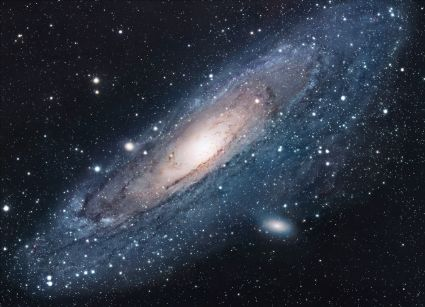
\includegraphics[scale=1.7]{universe}
\caption{The Universe}
\label{fig:universe}
\end{figure}

\section{Conclusion}
``I always thought something was fundamentally wrong with the universe'' \citep{adams1995hitchhiker}




\section{font}

The section num is \thesection

fi   f\mbox{}i

OK. That's fine.\\
OK\@. That's fine.

Prof. Smith is a nice man.\\
Prof.~Smith is a nice man.
\subsection{special character}
\XBox \male \female \phone \checked \twonotes

\begin{itemize}
    \item[+] first
    \item[*] second
    \item[\LaTeX] three
\end{itemize}
\begin{enumerate}
    \item first
    \item second
    \item three
\end{enumerate}

\subsection{underline}
\uline{line}
\uline{underline} \\
\uuline{double underline} \\
\dashuline{dash underline} \\
\dotuline{dot underline} \\
\uwave{wave} \\
\sout{delete} \\
\xout{deletex}

\textbf{BOLD?}
\textit{italy}
1-2
1--2
1---2
\ldots
\emph{pay attention}
\section{space control}

FFFFFFFFFFFFFFF

FFFFFFFFFaaaa

\subsection{magic space in par}

\fbox{first example}

{\parbox[t]{2em}{hahahaafdsfda}}

\fbox{second example}

{
\leftskip=3em
\parindent=1em
Here is for hang up in paragragh

hang on in paragraghs hhhhhhhhhhhhhhhhhhhhhhhhhhhhhhhhhhhhhhhhhhhhhhhhhhhhhhhhhhhhhhhhhhhhhhhhhhhhhhhhhhhhhhhhhhhhhhhh

two hhhhhhhhhhhhhhhhhhhhhhhhhhhhhhhhhhhhhhhhhhhhhhhhhhhhhhhhhhhhhhhhhhhhhhhhhhhhhhhhhhhhhhhhhhhhh

three

}

\section{mutlicolumn}
\fbox{third example}

	aaa\hspace{.25\textwidth}aaa
	
	\parbox[t]{5em}{TeXxxxxx xxxxxxxxxxxxxxxx xxxxxxxxxxxxxxxxxxxxxxxx           xxxxxxxxxxxxxxxxxxxxxxxxxxxxxxxxxxxxxx xxxxxxxxxxxxxxxxxx\par Tex}
	\hfill
	\parbox[t]{0.2\linewidth}{TeX\smallskip\par TeX}
	\hfill
	\parbox[t]{0.2\linewidth}{TeX\bigskip\par\ TeX}


This is \parbox[t]{4em}{an long
example to show} how \parbox[b]
{5em}{parbox' works perfectly.}

This is 
\begin{minipage}[t]{4em}
an long
example to show
\end{minipage}
how 
\parbox[b]
{5em}{parbox' works perfectly.}

\parbox[t]{0.25\linewidth}{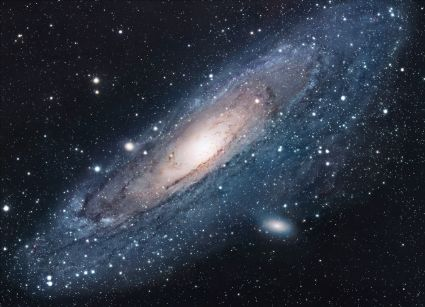
\includegraphics[scale=1.7]{universe.jpg}}
\hfill
\parbox[t]{0.25\linewidth}{zhuangyulin\par TEL;1865555555\par email:}

\section{footnote}

This is an example\footnote{haah}.

\begin{minipage}{0.2\linewidth}
This is an example \footnotemark
\footnotetext{haha}
\end{minipage}


\section{\fbox{Box}}
\rotatebox[origin=c]{90}{R}otate box

\raisebox{0.3em}{R}aisebox

\textcolor{red}{red}emphasis

\colorbox[gray]{0.85}{gray background box}

\fcolorbox{red}{pink}{
\textcolor{blue}{fancy frame box}
}

\LaTeX---\scalebox{3}[3]{\LaTeX scalebox}

\bibliographystyle{plain}
\bibliography{references}
\end{document}
